\documentclass[main.tex]{subfiles}
\begin{document}
\chapter{Off-line scheduling of parallel tasks}
\thispagestyle{chapstyle}
\label{chap_schedParallelTasks}
\minitoc

In this chapter, we investigate the methods to schedule parallel tasks off-line and we give a particular focus on approaches that can be applied to distributed architectures while meeting constraints~\ref{constr_schedOffLine} and~\ref{constr_scalability} detailed in Chapter~\ref{chap_systemModel}. We firstly overview in Section~\ref{sec_stateOfTheArt_2_DAGsched} the existing works that deal with \emph{DAG tasks}~\cite{Baruah2012_RTSS} since they have many similarities with our application model. We then focus on methods that have been proposed to schedule DAG tasks off-line on multi- and many-core processors. We will analyze methods based on off-line transformations of the model and approaches using complete off-line scheduling of the tasks. Finally, we will detail the solutions that were proposed to tackle hard real-time mapping problems on distributed architectures. 

\section{Off-line scheduling of DAG tasks}
\label{sec_stateOfTheArt_2_DAGsched}

The \emph{Directed Acyclic Graph} (or \emph{DAG}) model is often considered as the most general model for tasks with explicit parallelism~\cite{Baruah2012_RTSS}. Indeed most of other parallel task models such the Fork-join~\cite{Lakshmanan2010} and the Parallel Synchronous~\cite{Saifullah2011} models can be seen as special cases of the DAG model.

\subsection{DAG model}
 A periodic DAG task is modeled as a set of sub-tasks whose execution order is constrained by precedence relations. Studying the DAG model is relevant in our case since its suits very well one part of our problem, namely the precedence constraints between sub-tasks. However, one may note that our model is more expressive than a pure DAG because communications between sub-tasks are made explicit as well as the transactions targeting external memories. A real-time DAG task is periodically activated and must complete before an implicit deadline. Usually, all sub-tasks are activated with their parent task and temporally constrained with the same deadline. More precisely, a taskset is modeled as $\tau = \{ \tau_1 , \ldots , \tau_n \}$ with $\tau_i = <S_i, P_i, T_i>$ a DAG task characterized by:
        $S_i = \{ \tau_i^1 , \ldots , \tau_i^{n_i} \}$ the set of sub-tasks, 
        $P_i \subset S_i \times S_i$ the set of precedence relations between the sub-tasks and 
        $T_i$ the period of the task. Each sub-task $\tau_i^j$ is associated with its WCET $C_i^j$. An example of DAG task is depicted in Figure~\ref{fig_stateOfTheArt_2_DAGTask}. A DAG task can be seen as a directed graph~\cite{BangJensen2008} $G = <N,E>$ where the \emph{nodes} $N = S = \cup S_i$ and the precedence relations are the \emph{edges} $E \subset N \times N$.

\begin{figure}
    \centering
    
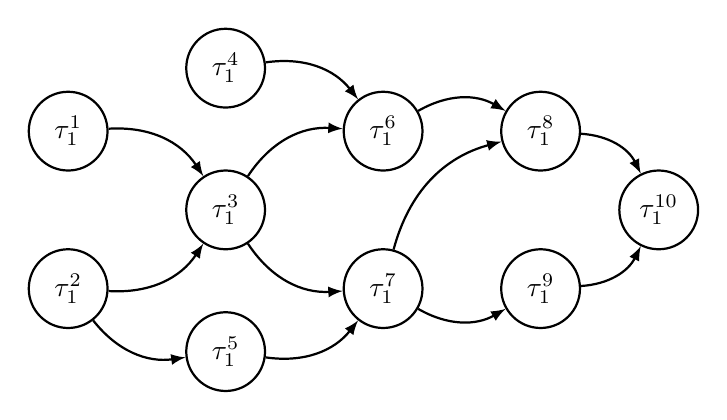
\begin{tikzpicture}[font={\fontsize{10pt}{12}\selectfont}]

\draw (0,1) node[circle, draw, thick, inner sep=0pt, minimum width=1cm] (t11) {$\tau_1^1$};
\draw (0,-1) node[circle, draw, thick, inner sep=0pt, minimum width=1cm] (t12) {$\tau_1^2$};

\draw (2,0) node[circle, draw, thick, inner sep=0pt, minimum width=1cm] (t13) {$\tau_1^3$};

\draw (2,1.8) node[circle, draw, thick, inner sep=0pt, minimum width=1cm] (t14) {$\tau_1^4$};
\draw (2,-1.8) node[circle, draw, thick, inner sep=0pt, minimum width=1cm] (t15) {$\tau_1^5$};

\draw (4,1) node[circle, draw, thick, inner sep=0pt, minimum width=1cm] (t16) {$\tau_1^6$};
\draw (4,-1) node[circle, draw, thick, inner sep=0pt, minimum width=1cm] (t17) {$\tau_1^7$};

\draw (6,1) node[circle, draw, thick, inner sep=0pt, minimum width=1cm] (t18) {$\tau_1^8$};
\draw (6,-1) node[circle, draw, thick, inner sep=0pt, minimum width=1cm] (t19) {$\tau_1^9$};

\draw (7.5,0) node[circle, draw, thick, inner sep=0pt, minimum width=1cm] (t110) {$\tau_1^{10}$};


\draw[-latex, thick, bend left] (t11) edge node {} (t13);
\draw[-latex, thick, bend right] (t12) edge node {} (t13);
\draw[-latex, thick, bend right] (t12) edge node {} (t15);

\draw[-latex, thick, bend left] (t14) edge node {} (t16);
\draw[-latex, thick, bend right] (t15) edge node {} (t17);

\draw[-latex, thick, bend left] (t13) edge node {} (t16);
\draw[-latex, thick, bend right] (t13) edge node {} (t17);

\draw[-latex, thick, bend left] (t16) edge node {} (t18);
\draw[-latex, thick, bend left] (t17) edge node {} (t18);
\draw[-latex, thick, bend right] (t17) edge node {} (t19);

\draw[-latex, thick, bend left] (t18) edge node {} (t110);
\draw[-latex, thick, bend right] (t19) edge node {} (t110);
\end{tikzpicture}

    \caption{Example of a DAG task $\tau_1$ with 10 sub-tasks}
    \label{fig_stateOfTheArt_2_DAGTask}
\end{figure}


We will firstly introduce classical DAG notions to ease the understanding of the following sections. Then, we will study the founding contributions on DAG scheduling on mono-core processors before analyzing the extensions that were made more recently for multi-core chips.

\subsection{DAG notions}
DAGs inherit from all the theoretical foundations of Graph Theory~\cite{BangJensen2008}. Manipulation of DAGs are commonly achieved using classical mathematical notions on directed graphs. For commodity, we remind some of these notions and precise the notations below.

A \emph{path} is a sequence of adjacent nodes defined as $p = <n_1 , \ldots , n_k>$. $p$ connects $n_1$ to $n_k$ if and only if subsequent nodes are connected by edges in $E$, i.e, 

\begin{displaymath}
\forall i \in [1, k-1] , (n_i, n_{i+1}) \in E
\end{displaymath}


The \emph{parents} of a node $n_i \in N$  are the set of nodes connected to $n_i$ by an edge and preceding it in the ordering. More precisely, $n_j$ is a parent of $n_i$ if and only if $ (n_j, n_i) \in E$. Similarly, the \emph{children} of $n_i$ are the set of nodes connected to $n_i$ by an edge and following it in the ordering. More precisely, $n_j$ is a child of $n_i$ if and only if $ (n_i, n_j) \in E$. For commodity, let us define the following notations:

\begin{displaymath}
    Parents ( n_i ) := \{ \; n_j \; | \; \forall (n_j,n_i) \in E \; \}
\end{displaymath}
\begin{displaymath}
    Children ( n_i ) := \{ \; n_j \; | \; \forall (n_i,n_j) \in E \;\}
\end{displaymath}

\begin{example}[Parents and children in DAGs]
    The parents of the sub-task $\tau_1^7$ in Figure~\ref{fig_stateOfTheArt_2_DAGTask} are $\tau_1^3$ and $\tau_1^5$. Its children are $\tau_1^8$ and $\tau_1^9$.
\end{example}

The \emph{predecessors} of a node extend the notion of parents recursively. $n_j$ is a predecessor of $n_i$ if and only if there is a path linking $n_j$ to $n_i$. Similarly, the \emph{successors} of a node extend the notion of children recursively. $n_j$ is a successor of $n_i$ if and only if there is a path linking $n_i$ to $n_j$. Let us define the following notations:


\begin{displaymath}
    Preds ( n_i ) := Parents (n_i) \underset{n_j \in Parents(n_i)}{\bigcup} Preds (n_j)
\end{displaymath}
\begin{displaymath}
    Succs ( n_i ) := Children (n_i) \underset{n_j \in Children(n_i)}{\bigcup} Succs (n_j)
\end{displaymath}


\begin{example}[Predecessors and successors in DAGs]
    The predecessors of the sub-task $\tau_1^7$ in Figure~\ref{fig_stateOfTheArt_2_DAGTask} are $\tau_1^1, \tau_1^2, \tau_1^3$ and $\tau_1^5$. Its successors are $\tau_1^8, \tau_1^9$ and $\tau_1^{10}$.
\end{example}

The notions of \emph{entry} and \emph{exit} sub-tasks in a DAG refer respectively to sub-tasks having no predecessors and sub-tasks having no successors.


The \emph{Critical Path} (or $CP$) in a DAG is its longest \emph{sequential} path. The length a path in a DAG task model is equal to the sum the WCETs of sub-tasks composing it. The $CP$ of a DAG task represents a lower-bound on the execution time of the task when fully parallelized. The ratio between the WCET of the task and the length of its CP is defined as the \emph{maximum speedup} $M$ \cite{Hill2008}.

\begin{displaymath}
    M(\tau_i) = \dfrac{ \underset{\tau_i^j \in S_i}{\sum} C_i^j}{ \underset{ \tau_i^k \in CP(\tau_i) }{\sum} C_i^k}
\end{displaymath}

\begin{example}[CP and speedup]
    Assuming that odd sub-tasks of Figure~\ref{fig_stateOfTheArt_2_DAGTask} 
    ($\tau_1^1 , \tau_1^3, \tau_1^5, \tau_1^7$ and $\tau_1^9$) have a WCET of 5 and the even sub-tasks 
    ($\tau_1^2 , \tau_1^4, \tau_1^6, \tau_1^8$ and $\tau_1^{10}$) have a WCET of 3, the critical path of the task is $CP(\tau_1) = <\tau_1^1 , \tau_1^3, \tau_1^7, \tau_1^9 , \tau_1^{10}>$ with a length of 23. The total WCET of $\tau_1$ is 40. Thus, $M(\tau_1) = 40/23 \simeq 1.74$. 
\end{example}

DAG nodes can be sorted in a \emph{topological order} to produce a linear sequence of sub-tasks that respect the precedence constraint.

\begin{example}[Topological order]
    A topological order of the DAG of Figure~\ref{fig_stateOfTheArt_2_DAGTask} is:
    $$< \tau_1^1 , \tau_1^2 , \tau_1^4 , \tau_1^5, \tau_1^3 , \tau_1^7 , \tau_1^6 , \tau_1^8 , \tau_1^9 , \tau_1^{10} >$$
\end{example}

Topological sorting is of importance since its provides a correct mono-core schedule of a DAG task. Algorithms are known to produce topological ordering of any DAG in linear time.\\



\subsection{Off-line model transformation}
Chetto \etal presented in~\cite{Chetto1990} an approach to schedule independent periodic sequential tasks together with sporadic groups of DAG tasks on \emph{mono-core} processors. Chetto \etal proposed to modify the timing parameters of the constrained sub-tasks to transform them in an equivalent set of independent tasks that can be scheduled with classical algorithms such as EDF. The idea is to assign each sub-task in the DAG a modified release date based on the finish time of its parents and a modified deadline based on the deadline of its children.
In~\cite{Chetto1990}, only one DAG task in considered. Each sub-task $\tau_i^j$ is also provided together with an activation date (or \emph{offset}) $s_i^j$ and a relative deadline $d_i^j$. The idea is to replace the precedence relations $P_i$ by changing the $s_i^j$ and $d_i^j$ parameters of each sub-task. We denote the modified parameters $ \widetilde{s_i^j}$ and $ \widetilde{d_i^j} $.
 Deadlines are adjusted as follows:
\begin{enumerate}
    \item For all tasks with no successors : $\widetilde{d_i^j} := d_i^j$;
    \item Select a task for which all children are already assigned an adjusted deadline;
    \item For the selected sub-task $\tau_i^j$: 
        \begin{displaymath}
            \widetilde{d_i^j} := \min ( \; d_i^j \; , \; \underset{\forall \tau_i^k \in children(\tau_i^j)}{\min} ( \widetilde{d_i^k} - C_i^k) \; )
        \end{displaymath}
    \item Repeat step 2 and 3 while there are tasks with unadjusted deadlines.
\end{enumerate}
In a symmetric manner, the activation dates are adjusted as follows:
\begin{enumerate}
    \item For all tasks with no predecessors : $ \widetilde{s_i^j} := s_i^j$;
    \item Select a task for which all parents have adjusted activation dates;
    \item For the selected task $\tau_i^j$:
        \begin{displaymath}
            \widetilde{s_i^j} := \max ( \; s_i^j \; , \; \underset{\forall \tau_i^l \in parent(\tau_i^j)}{\max} \; \widetilde{s_i^k} + C_i^k) \; )
        \end{displaymath}
    \item Repeat step 2 and 3 while there are tasks with unadjusted activation dates.
\end{enumerate}
The process of adjusting timing parameter is achieved prior to execution of the tasks. Once all tasks have updated timing parameters, they can be considered as independent. Thus, they can be scheduled on-line using classical scheduling algorithm taking into account offsets and constrained deadlines. 

\begin{example}[Modification of timing parameters]
    Let us consider 10 sub-tasks $\{ \tau_1^1 , \ldots , \tau_1^{10} \}$ constrained by the precedence relations depicted in Figure~\ref{fig_stateOfTheArt_2_DAGTask}. Table~\ref{table_stateOfTheArt_2_exampleChettoDAG} shows an example of modified timing parameters for the 10 sub-tasks following the algorithm described in~\cite{Chetto1990}.

\begin{table}
\centering
\begin{tabular*}{0.7\linewidth}{@{\extracolsep{\fill}} c c c c c c c}
    \hline
    Sub-task        & $s_1^i$   & $C_1^i$   & $d_1^i$   & $T_1^i $  & $\widetilde{s_1^i}$   & $\widetilde{d_1^i}$ \\
    \hline
     $\tau_1^1$  & 0         & 3         & 40        & 40        & 0                     & 25 \\
     $\tau_1^2$  & 0         & 4         & 40        & 40        & 0                     & 25 \\
     $\tau_1^3$  & 0         & 2         & 40        & 40        & 4                     & 27 \\
     $\tau_1^4$  & 0         & 6         & 40        & 40        & 0                     & 28 \\
     $\tau_1^5$  & 0         & 1         & 40        & 40        & 4                     & 40 \\
     $\tau_1^6$  & 0         & 3         & 40        & 40        & 6                     & 31 \\
     $\tau_1^7$  & 0         & 4         & 40        & 40        & 6                     & 31 \\
     $\tau_1^8$  & 0         & 6         & 40        & 40        & 10                    & 37 \\
     $\tau_1^9$  & 0         & 5         & 40        & 40        & 10                    & 37 \\
     $\tau_1^{10}$ & 0       & 3         & 40        & 40        & 16                    & 40 \\
	\hline	
\end{tabular*}
\caption{Example of adjusted timing parameters for DAG tasks using the algorithm described in~\cite{Chetto1990}}
\label{table_stateOfTheArt_2_exampleChettoDAG}
\end{table}

\end{example}

The authors proved the optimality of this algorithm in the sense that the original dependent task set is schedulable if and only if the modified taskset is schedulable using a preemptive scheduling algorithm. However, scheduling tasks with offsets in a non-preemptive manner, even without precedence constraints remains NP-hard~\cite{Lenstra1977}. And similarly, Ullman showed in~\cite{Ullman1975} that, in a \emph{multi-core} context, scheduling DAG tasks is also strongly NP-Hard, even using a preemptive algorithms. \\ 

In a similar approach, Qamieh \etal~\cite{Qamhieh2013, Qamhieh2014} adapted the method of~\cite{Chetto1990} to multi-core processors using the \emph{DAG stretching algorithm}. The idea of is to append as many non-critical sub-tasks as possible to the critical path to form one sequential thread with a maximum utilization. By doing so, the number of sub-tasks that are executed in parallel with this main thread is minimized. The precedence relations of sub-tasks executed in parallel to the main thread are enforced using adjusted timing parameters as in~\cite{Chetto1990}. The modified taskset is then scheduled online using GEDF. In~\cite{Qamhieh2014}, Qamieh \etal showed in simulation with synthetic tasksets that, despite the goal of minimizing the parallelism during execution, this approach had better schedulability ratios than existing techniques for scheduling DAG tasks. Yet, it can be argued that minimizing the slack of the master thread increases the risk of suffering deadline misses if the WCET estimation of a sub-task was inaccurate. \\

Many of the other contributions on the multi-core scheduling of DAG tasks, including~\cite{Baruah2012_RTSS}, \cite{Li13} and \cite{Bonifaci2013} are based on pure on-line scheduling techniques and thus out of the scope of this thesis.


%In~\cite{Qamhieh2013, Qamhieh2014}, Qamieh \etal emphasized that the authors of~\cite{Baruah2012_RTSS,Li13,Bonifaci2013} were only considering \emph{general} timing parameters of DAG tasks such as their total WCET or the length of their critical path. They argued that schedulability analysis of DAG tasks could be improved by taking into account more information about the timing parameters of sub-tasks and the constraints on their execution flow.
%They proposed two approaches denoted as the \emph{Model Transformation} and the \emph{Direct Scheduling} techniques for scheduling DAG tasks on multi-core processors. The idea of the Model Transformation is to convert each DAG task into a set of independent sequential tasks by adding extra timing parameters such as intermediate offsets and deadlines to sub-tasks. By doing so, the resulting modified taskset becomes a classical model of independent real-time tasks that can be scheduled using state-of-the-art algorithms.
%Yet, the Model Transformation technique has the drawback of losing some of the DAG model's generality and to become more restricted because of the extra timing parameters. To overcome this issue, the Direct Scheduling approach does not aim at modifying the model to re-use existing algorithms but rather to apply scheduling techniques directly on the DAG models without changing their characteristics. Globally, the idea of the \emph{DAG stretching algorithm} that implements the Direct Scheduling approach is to append as many non-critical sub-tasks as possible to the critical path to form one sequential thread with a maximum utilization. By doing so, the number of sub-tasks that are executed in parallel with this main thread is minimized, thus simplifying the scheduling. In~\cite{Qamhieh2014}, Qamieh \etal showed in simulation with synthetic tasksets that, despite the goal of minimizing the parallelism during execution, this approach had better schedulability ratios than existing techniques for scheduling DAG tasks. Yet, it can be argued that minimizing the slack of the master thread increases the risk of suffering deadline misses if the WCET estimation of a sub-task was inaccurate.






\subsection{Off-line mapping of DAGs on multi-core}


\subsubsection{Real-time scheduling}



The problem of mapping off-line dependent tasksets on multi-core processors has already been addressed in the real-time community. Grolleau and Choquet-Geniet~\cite{Grolleau2001} proposed a technique based on Petri nets to compute such mappings. They fully model the tasks and the execution target with Petri nets augmented by a constraint on the largest number of transitions crossed simultaneously as shown in Figure~\ref{fig_stateOfTheArt_2_taskPetriNet}. This approach allows both preemption and migration of tasks between cores of the processor. The schedule is computed with the Petri nets and the mapping is done afterwards in post-processing in order to minimize the number of migrations. Overall, this approach provides a formal solution to the scheduling problem and can provide optimal results regarding different performance criteria (shortest response time, balance of idle periods, ...). However, the scalability of Petri nets on that kind of problem is questionable and the approach needs to be evaluated over large applications. 

\begin{figure}
    \centering
    %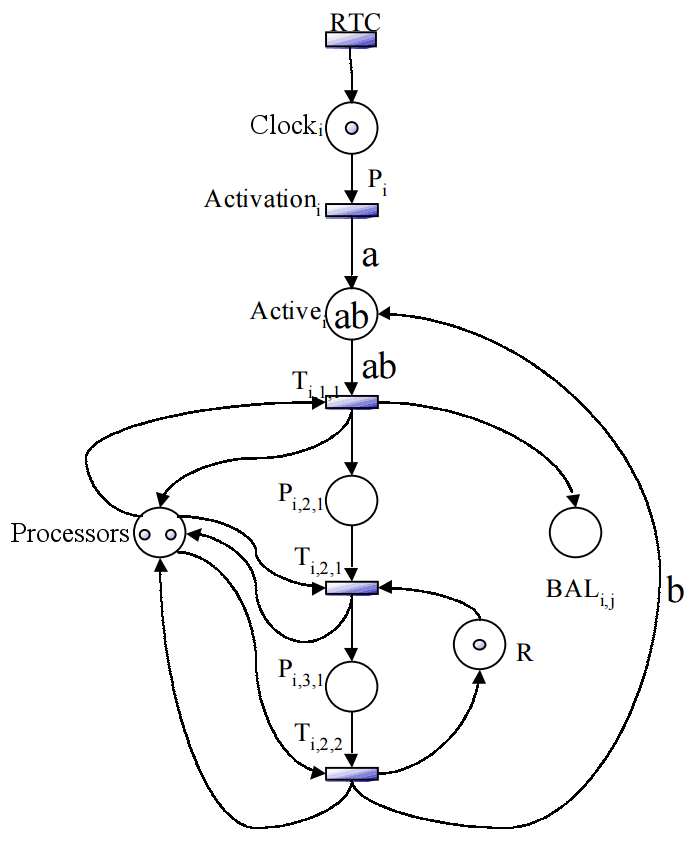
\includegraphics[height=10cm]{imgs/png/stateOfTheArt_2_taskPetriNet.png}
    \scalebox{0.9}{
% X, Y, PRINTNAME, LABEL
\newcommand\petritrans[4]{
    \node[rectangle, draw, color=black, fill=gray, thick, inner sep=0pt, minimum width=0.2cm, minimum height=1cm] (#4) at (#1,#2) {};
    \draw (#1,#2+0.8) node {#3};
}

% X, Y, PRINTNAME, LABEL, INSIDESTUFF
\newcommand\petrinode[5]{
    \node[circle, draw, color=black, thick, inner sep=0pt, minimum size=1cm] (#4) at (#1,#2) { #5 };
    \draw (#1,#2+0.8) node {#3};
}

% X, Y
\newcommand\petrijeton[2]{
    \node[circle, draw,  color=black, fill=gray, thick, inner sep=0pt, minimum size=0.2cm] (test) at (#1,#2) {};
}

\begin{tikzpicture}[font={\fontsize{12pt}{12}\selectfont}]

    \petritrans{0}{0}{RTC}{rtc}
    \petrinode{2}{0}{Clock$_i$}{clk}{}
    \petrijeton{2}{0}

    \petritrans{4}{0}{Activation$_i$}{activation}
    \petrinode{6}{0}{Active$_i$}{active}{ab}
    
    \petritrans{8}{0}{T$_{i,1,1}$\hspace{0.6cm} }{Ti11}
    \petrinode{10}{0}{P$_{i,2,1}$}{Pi21}{}
    
    \node[circle, draw, color=black, thick, inner sep=0pt, minimum size=1cm] (procs) at (10,-3) {  };
    \draw (10,-3.8) node {Processors};
    \petrijeton{9.85}{-3}
    \petrijeton{10.15}{-3}
    
    \petrinode{10}{2}{BAL$_{i,j}$}{BALij}{}


    \petritrans{12}{0}{T$_{i,2,1}$\hspace{0.9cm} }{Ti21}
    \petrinode{14}{0}{P$_{i,3,1}$}{Pi31}{}
    
    \petrinode{13.5}{2}{R}{R}{}
    \petrijeton{13.5}{2}
    
    
    \petritrans{16}{0}{\hspace{1.2cm}T$_{i,2,2}$}{Ti22}


    \draw[-latex, thick] (rtc) edge node {} (clk);
    \draw[-latex, thick] (clk) edge node[below] {P$_i$} (activation);
    \draw[-latex, thick] (activation) edge node[below] {a} (active);
    \draw[-latex, thick] (active) edge node[below] {ab} (Ti11);
    \draw[-latex, thick] (Ti11) edge node {} (Pi21);
    \draw[-latex, thick] (Pi21) edge node {} (Ti21);
    \draw[-latex, thick] (Ti21) edge node {} (Pi31);
    \draw[-latex, thick] (Pi31) edge node {} (Ti22);
    
    \draw[-latex, thick, bend left] (Ti11) edge node {} (BALij);
    \draw[-latex, thick, bend left] (Ti11) edge node {} (procs);

    \draw[-latex, thick, bend left] (Ti21) edge node {} (procs);


    \draw[-latex, thick, bend right] (Ti22) edge node {} (R);
    \draw[-latex, thick, bend right=100, above] (Ti22) edge node {b} (active);
    \draw[-latex, thick, bend left=50] (Ti22) edge node {} (procs);

    \draw[-latex, thick, bend right] (R) edge node {} (Ti21);
    
    \draw[-latex, thick, bend left] (procs) edge node {} (Ti11);
    \draw[-latex, thick, bend left] (procs) edge node {} (Ti21);
    \draw[-latex, thick, bend right=30] (procs) edge node {} (Ti22);
\end{tikzpicture}
}
    \caption{Example of task modeled using Petri nets}
    \label{fig_stateOfTheArt_2_taskPetriNet}
\end{figure}

Unfortunately, several other formal approaches to this problem such as the work on Priced Timed Automata of Behrmann \etal~\cite{Behrmann2005} or the {\sc Uppaal} formulation of Baro \etal~\cite{Baro2012} also face major scalability issues.\\

In~\cite{Boniol2008}, Boniol \etal tackled the scalability issue by using an approach based on \emph{Constraint Programming}. They rely on an AER-like execution model (Section~\ref{ssec_stateOfTheArt_softwareEnforcedPredictability}) where tasks are run on a bus-based multicore processor. Each task is split in \emph{execution} and \emph{communication} slices. The mapping problem is thus turned into a slice assignment problem of where each core is modeled by a series of execution slots of equal lengths and the shared bus is also modeled by communication slots having the same length. The problem is then to assign execution slices to core slots and communication slices to bus slots. CPU utilization is constrained by checking that the sum of the WCET of execution slices assigned to a slot is not superior to the length of the slot. Precedences are enforced using constraints on the position of the slots to which execution slices are assigned. Similar constraints are provided to account for memory and communication limitations. Although not directly applicable to a many-core processor and thus to our problem, such an approach based on Constraint Programming seems to be capable of scaling up to industrial-sized problems. This demonstrated scalability was one of the main reasons for investigating solution based on Constraint Programming when designing our mapping tool as described in Chapter~\ref{chap_budgetValidation}.



\subsubsection{Makespan-optimization}
Outside from the real-time community, the problem of scheduling off-line dependent tasksets on multi-core processors has been thoroughly studied. As a main difference, the tasks models that are commonly considered do not necessarily represent periodic tasks or include any deadline constraints. In general, the approaches rather strive for reducing the total completion time of a DAG task, commonly referred to as the \emph{makespan-optimization} problem.

\begin{definition}[Makespan]
    The makespan is the time difference between the beginning of the first running sub-task and the end of the last running sub-task in a specific schedule. The optimal (shortest) makespan of a task is equal to the length of its critical path.
\end{definition}

In~\cite{Kwok1999}, Kwok and Ahmad overviewed the plethora of static scheduling algorithms for allocating non-periodic DAG tasks on multi-core processor. Given the NP-completeness of the scheduling problem~\cite{Garey1979}, most of the proposed solutions consider heuristics based on the \emph{list scheduling} technique~\cite{Adam1974,Ahmad1996,Casavant1988,ElRewini1994,Gerasoulis1992,Shirazi1990,McCreary1994,Yang1988,Coffman1976}. The idea is to keep a priority queue of the sub-tasks that can be scheduled and to iteratively pick $\tau_i^j$ the first element of the queue, place it on the core on which it can start the earliest and add to the queue the children sub-tasks of $\tau_i^j$. Usually, the scheduling algorithms vary essentially in the way of assigning priorities to sub-tasks. 


Some algorithms assign static priorities to sub-tasks such as \emph{HLF} (or \emph{Highest Level First})~\cite{Coffman1976}, \emph{LPT} (or \emph{Longest Processing Time})~\cite{Friesen1987} and \emph{CP} (or \emph{Critical Path})~\cite{graham1979}. More recent approaches usually assign priorities \emph{dynamically}. In these approaches, the priorities are not fixed a priori and all priorities in the scheduling queue are re-computed every time a sub-task is appended to it.  

Two common timing attributes for assigning priorities to sub-tasks are the \emph{b-level} and the \emph{t-level} defined as:
\begin{description}
    \item[t-level] : the t-level of a sub-task $\tau_i^j$ is the longest path from an entry node to $\tau_i^j$. The t-level can be seen as the earliest start time of a sub-task.
    \item[b-level] : the b-level of a sub-task $\tau_i^j$ is the longest path from $\tau_i^j$ to an exit node. All b-levels are upper bounded by the length of the Critical Path of the DAG.
\end{description}

These timing attributes are used in many popular list-scheduling algorithms such as the \emph{Highest Level First with Estimated Times} (or \emph{HLFET}) algorithm~\cite{Adam1974}, the \emph{Insertion Scheduling Heuristic} (or \emph{ISH})~\cite{Kruatrachue1987} or the \emph{Modified Critical Path} (or \emph{MPC}) algorithm~\cite{Wu1990}. A description of HLFET is provided in Algorithm~\ref{algo_stateOfTheArt_2_HLFET}. 


\begin{algo}[HLFET] 
    \hfill
    \begin{enumerate}
        \item Compute the \emph{b-level} of each sub-tasks
        \item Put ready sub-tasks into the priority queue. Highest priority is given to sub-tasks with largest b-level.
        \item Schedule the sub-task with highest priority to the core on which it can start the earliest.
        \item Update the scheduling queue with the sub-tasks that are now ready.
        \item Repeat 3 and 4 until all sub-tasks are scheduled.
    \end{enumerate}
    \label{algo_stateOfTheArt_2_HLFET}
\end{algo}


\begin{example}[Application of HLFET]
Let us consider 10 sub-tasks $\{ \tau_1^1 , \ldots , \tau_1^{10} \}$ constrained by the precedence relations depicted in Figure~\ref{fig_stateOfTheArt_2_DAGTask}. The WCETs of the sub-tasks are those defined in Table~\ref{table_stateOfTheArt_2_exampleChettoDAG}. Periods and offsets are ignored. Table~\ref{table_stateOfTheArt_2_exampleScheduleHLFET} shows an example of b-level, start dates ($\widetilde{s_1^i}$) and core ($c_i$) assignment of sub-tasks when using HLFET on a dual-core target. The two cores are denoted $c_1$ and $c_2$. As depicted in Figure~\ref{fig_stateOfTheArt_2_exampleScheduleHLFET}, the makespan of this schedule is 21.

\begin{figure}
    \centering
    \tikzset{timing/.append style={x=3ex, y=2.5ex}}
    
\begin{tikztimingtable}[timing/lslope=0, timing/slope=0, timing/coldist=0.8, timing/d/text/.append style={font=\rmfamily}, timing/d/background/.style={fill=white} ]
    $c_1$ & 0.01L 3D{$\tau_1^1$} 6D{$\tau_1^4$} 3D{$\tau_1^6$} [fill=lightgray]6D{$\tau_1^8$} [fill=white]3L\\
    $c_2$ & 0.01L [fill=lightgray]4D{$\tau_1^2$} 2D{$\tau_1^3$} [fill=white]1D{$\tau_1^5$} [fill=lightgray]4D{$\tau_1^7$} [fill=white]5D{$\tau_1^9$} [fill=white] 2S [fill=lightgray]3D{$\tau_1^{10}$} [fill=white]0.01L \\
\extracode
    \draw[-latex] (0, -2) -- (22, -2);
    \draw[-latex] (0, 0) -- (22, 0);
    \Cote[-8mm]{(0,-2)}{(21,-2)}{ \small \rmfamily \emph{Makespan = 21} }<h>
\begin{background}
    \vertlines[dashed]{}
\end{background}
\end{tikztimingtable}

    \caption{Example of schedule produced by HLFET on two cores. The sub-tasks of the critical path are colored in gray.}
    \label{fig_stateOfTheArt_2_exampleScheduleHLFET}
\end{figure}


\begin{table}
\centering
\begin{tabular*}{0.7\linewidth}{@{\extracolsep{\fill}} c c c c}
    \hline
     Sub-task        & b-level   & $\widetilde{s_1^i}$   & Core \\
    \hline
     $\tau_1^1$  & 18         & 0         & $c_1$        \\
     $\tau_1^2$  & 19         & 0         & $c_2$        \\
     $\tau_1^3$  & 15         & 4         & $c_2$        \\
     $\tau_1^4$  & 18         & 3         & $c_1$        \\
     $\tau_1^5$  & 14         & 6         & $c_2$        \\
     $\tau_1^6$  & 12         & 9         & $c_1$        \\
     $\tau_1^7$  & 13         & 7         & $c_2$        \\
     $\tau_1^8$  & 9         & 12         & $c_1$        \\
     $\tau_1^9$  & 8         & 11         & $c_2$        \\
     $\tau_1^{10}$ & 3       & 18         & $c_2$        \\
	\hline	
\end{tabular*}
\caption{Example of schedule produced by HLFET on two cores}
\label{table_stateOfTheArt_2_exampleScheduleHLFET}
\end{table}

\end{example}


Overall, all those makespan-oriented scheduling algorithms consider single task problems without real-time constraints. Many heuristics have been proposed, mostly using a list-scheduling approach, in order to assign sub-tasks to cores. Yet, applying such approaches is impossible in a hard-real time context without profound modifications of the models and algorithms to manage multiple parallel tasks with deadline constraints. Moreover, these techniques usually don't apply to many-core architectures with distributed memory schemes since communications must be achieved explicitly by software and that both the cores and the NoC should be treated during the scheduling phase. For this reason, we explore in the next sections the contributions that were made regarding the scheduling of parallel tasks on such distributed architectures.



\section{Off-line mapping on distributed architectures}

In the previous section, we overviewed the approaches that have been proposed to map DAG tasks on multi-core processors. Yet, although providing good results, these approaches are usually not applicable to many-core targets such as the \mppalong. 
Indeed, the communications on multi-cores rely on shared memory while using NoC-based many-core processors requires to manage explicit communications using message-passing techniques when distributing an application over the whole chip. In this section, we overview the work that has been done to map real-time applications on the \mppalong, on other many-core processors and also more general (but still relevant) work on time-triggered macroscopic-sized distributed systems. 

\subsection{Mapping on the \mppalong}

In~\cite{Giannopoulou2015}, Giannopoulou \etal propose a \emph{mixed-criticality} scheduling policy for the \mppalong based on the \emph{Flexible Time-Triggered Scheduling} policy (or \emph{FTTS}) originally introduced in~\cite{Giannopoulou2013_EMSOFT}. A FTTS schedule consists of succession of \emph{frames} of fixed duration. The sequence of frames is repeated over a \emph{scheduling cycle} whose length equals the hyperperiod of the taskset. Each frame is composed of several \emph{sub-frames} of variable length during which tasks can execute. In a frame, tasks of high criticality levels are assigned to the firsts sub-frames while lower-criticality tasks are assigned ending sub-frames. By doing so, high-criticality tasks can be executed easily. Lower-criticality tasks coming after can be either fully executed, executed in degraded mode or just canceled depending on the remaining time in the current frame. Doing so enables to guarantee the safe execution of high criticality tasks while introducing some flexibility to efficiently use the hardware resources. Yet, the underlying assumption behind the FTTS is that the WCET of tasks are in the same order of magnitude to minimize idle states within sub-frames.

\begin{example}[FTTS scheduling policy]
    Figure~\ref{fig_stateOfTheArt_2_FTTS} depicts 2 cycles of an FTTS schedule. Tasks with high priorities are colored in dark gray. Low-priority tasks are in light gray. During the first frame of the second cycle, task 1 executes for a long time, thus leading to the execution of task 4 in degraded mode to keep the total execution time within the span of frame 1. One may note that the division into no overlapping sub-frame is implemented using barriers.

\begin{figure}
    \centering
    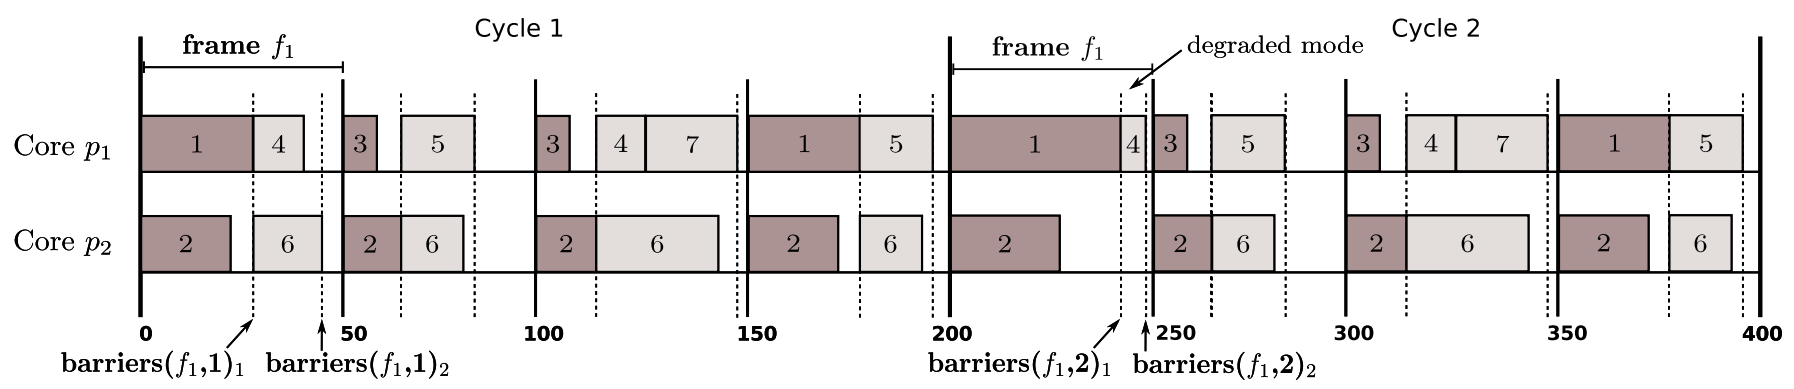
\includegraphics[width=15cm]{imgs/png/stateOfTheArt_2_FTTS.png}
    \caption{Example of FTTS schedule on 2 cycles (extracted from~\cite{Giannopoulou2015}).}
    \label{fig_stateOfTheArt_2_FTTS}
\end{figure}
\end{example}

In addition, in~\cite{Giannopoulou2015}, an analysis of the memory interferences inside compute cluster is proposed together with a method to compute WCTT of packets on the NoC using Network Calculus. Moreover, a mapping heuristic is detailed to optimize the utilization of cores, local memory banks and the NoC. Unfortunately, this work has not been implemented on any real target and still lacks experimental evaluation. Especially, the complexity of the run-time supporting the execution of frames and sub-frames is not detailed. \\

\begin{figure}
    \centering
    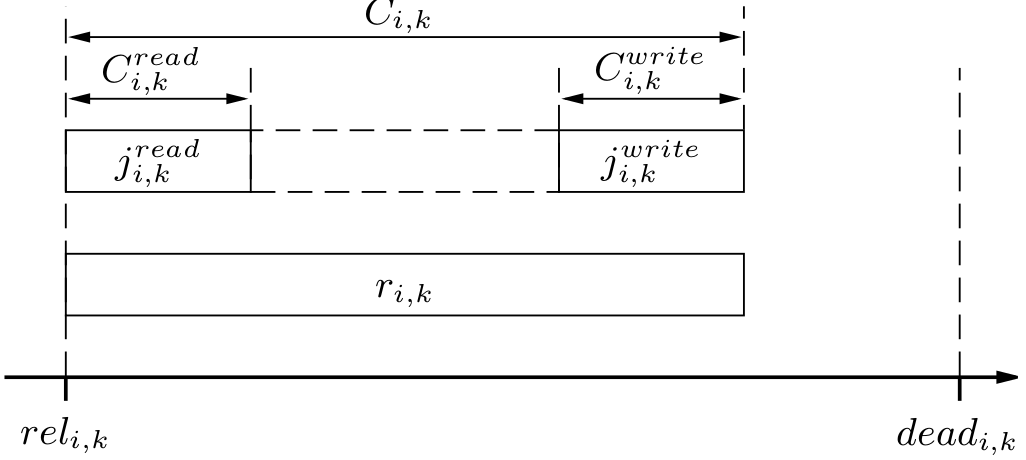
\includegraphics[width=10cm]{imgs/png/stateOfTheArt_2_RdWrExPhases.png}
    \caption{Read, write and execute phases of Runnables (extracted from~\cite{Becker16}).}
    \label{fig_stateOfTheArt_2_RdWeExPhases}
\end{figure}

In~\cite{Becker16}, Becker \etal proposed a method to schedule tasks inside a single cluster of the \mppalong. They proposed an ILP formulation of the mapping problem together with sub-optimal heuristics enabling the approach to scale from small programs to actual industrial-sized applications. The authors eliminated inter-core interferences during execution thanks to privatization of local memory banks to each core and assumed a \emph{read-execute-write} semantics of the application similar to the AER execution model previously described in Section~\ref{ssec_stateOfTheArt_softwareEnforcedPredictability}. They consider only automotive applications following an AUTOSAR model where each task $\tau_i$ (also denoted as a \emph{Runnable}) is a sequential piece of code characterized by a period $T_i$ , a WCET $C_i$ and memory footprint $S_i$. As shown in Figure~\ref{fig_stateOfTheArt_2_RdWeExPhases}, using the read-execute-write semantics, the WCET of a task is decomposed into three phases $C_i = C_i^{rd} + C_i^{ex} +C_i^{wr}$:
\begin{itemize}
    \item the read phase of duration $C_i^{rd}$ during which the code and data of the runnable are copied from the external RAM into a local cluster's memory bank;
    \item the execution phase of duration $C_i^{ex}$ during which the code of the task is executed by a PE;
    \item and the write phase of duration $C_i^{wr}$ during which the data produced by the task are committed to the external RAM.
\end{itemize}


In~\cite{Becker16}, the authors modeled each task by three jobs corresponding to the three phases. Then, they proposed different solutions to the problem of assigning execution jobs to cores and read and write jobs to non-overlapping time frames. In addition, communication between tasks are ensured using a dedicated local memory bank which statically stores all the data that will be exchanged. In doing so, the communication model of the application remains implicit and the  applicability of the approach is thus limited to single-cluster applications. In addition, bounds on $C_i^{rd}$ and $C_i^{wr}$ are computed while assuming no competing accesses to the external RAM thus limiting the applicability of the approach to the execution of at most 2 applications (1 per DDR-SDRAM controller). 



\subsection{Mapping on other many-core architectures}

\begin{figure}
    \centering
    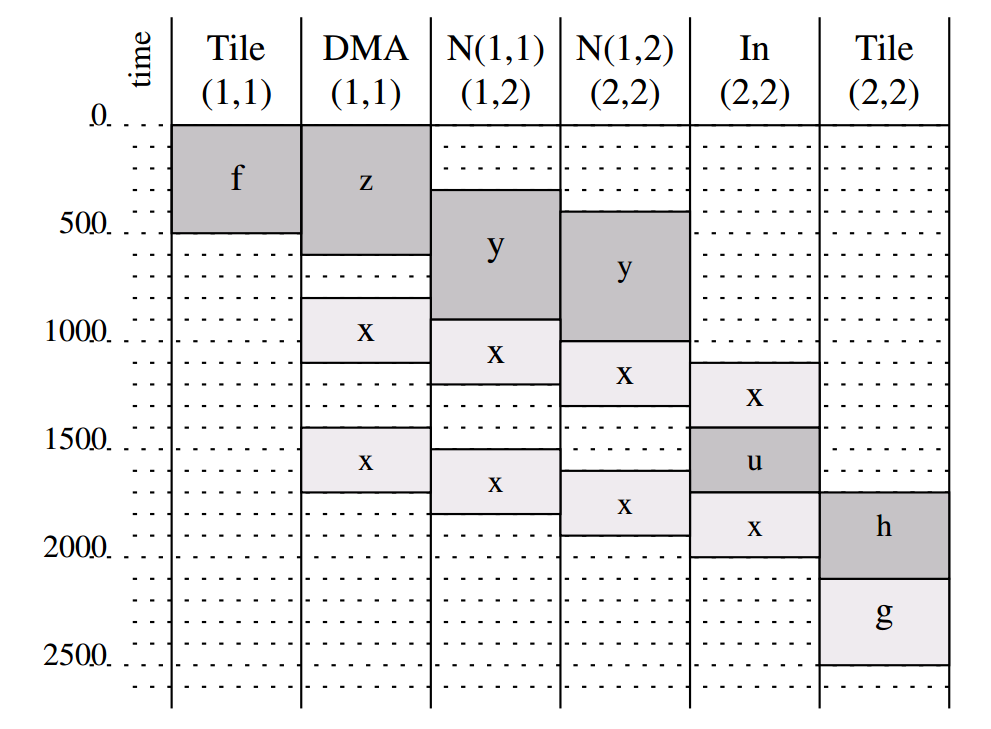
\includegraphics[width=9cm]{imgs/png/stateOfTheArt_2_LoPhTschedTable.png}
    \caption{Example of scheduling table produced by LoPhT (extracted from~\cite{Carle2014}).}
    \label{fig_stateOfTheArt_2_LoPhTschedTable}
\end{figure}

Carle \etal~\cite{Carle2014} proposed an efficient allocation and scheduling tool called \emph{LoPhT} for computing static mapping of dataflow applications on NoC-based many-core processors. They provide several heuristics computing global scheduling tables for tasks execution on cores and for communications on NoC resources in a time-triggered fashion. An example of such a scheduling table is depicted in Figure~\ref{fig_stateOfTheArt_2_LoPhTschedTable}. The approach is evaluated over an image processing application composed of 32 tasks and exhibits not only a correct execution regarding real-time bounds but also more generally improved performance and latency in comparison with hand-made parallelization. Unfortunately, several issues still need to be tackled for this approach to be applicable for our problem. Firstly only the case of one single DAG task is addressed and no support is provided for tasks with multiple periods. Secondly, accesses to external RAM are not taken into account. And finally, the feasibility still needs to be demonstrated with an implementation on a real target.\\ 


%Pagetti \etal presented the \emph{Research Open-Source Avionics and Control Engineering} (or \rosace) case study~\cite{Pagetti2014}. They describe a framework enabling the integration of real-time applications going from high level specifications in \emph{Simulink} down to the execution on many-core processors. They propose to translate the Simulink specification into several C programs assembled using \prelude~\cite{Pagetti2011} and to execute them in predictable manner on the target by the means of an execution model. However, although the \prelude compiler generates real-time parallel threads with precedence constraints, the main issue addressed in this paper is to demonstrate that an implementation respects the application's semantic and meets performance criteria at the system level. Thus, the process of mapping threads to core on the target is not addressed and is left to be done manually (at this stage) by the integrator. \\

\begin{figure}
    \centering
    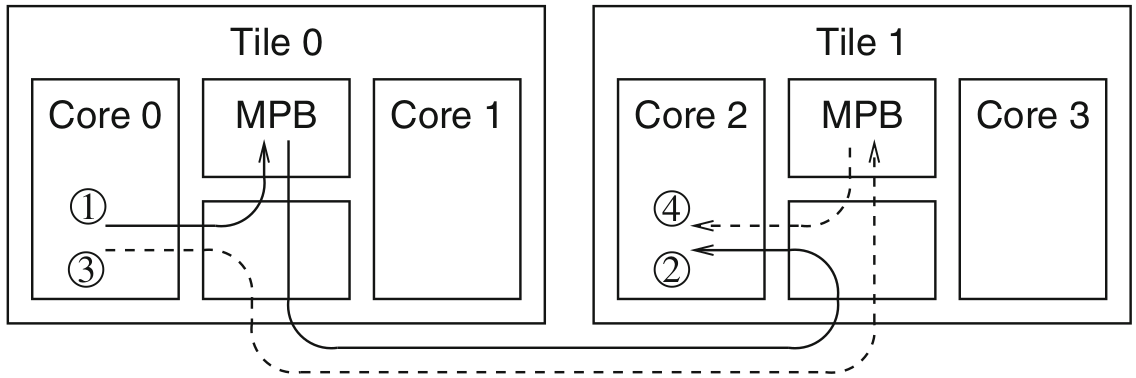
\includegraphics[width=10cm]{imgs/png/stateOfTheArt_2_pushPullSCC.png}
    \caption{Example of \emph{pull} (steps \circled{1} and \circled{2})  and \emph{push} (steps \circled{3} and \circled{4}) operations on the Intel SCC~\cite{intel_scc} (extracted from~\cite{PuffitschNP15}).}
    \label{fig_stateOfTheArt_2_pushPullSCC}
\end{figure}
In~\cite{PuffitschNP15}, Puffitsch \etal presented a method to map dependent tasksets on many-core platforms. They propose a general execution model enforcing predictable execution of applications, and they instantiate it for three different hardware platforms: the Intel SCC~\cite{intel_scc}, the Texas Instrument TMS320C6678~\cite{TMS320C6678} and the Mellanox TILEmpower-Gx36~\cite{TileGx36}. In addition, they provide a CP-based approach to map ``\emph{reasonably large}'' tasksets with extended precedence constraints on the three targets, thus enabling the utilization of a formal approach rather than sub-optimal heuristics for industrial-sized problems.
In~\cite{PuffitschNP15}, the authors assume time-bounded NoC communications relying on the notion of \emph{Message Passing Areas} (of \emph{MPAs}) inspired by the \emph{Message Passing Buffers} of the Intel SCC. In this model, tasks can either \emph{push} data in the remote MPA of another task or \emph{pull} data from a remote MPA into its local memory as shown in Figure~\ref{fig_stateOfTheArt_2_pushPullSCC}. The time required for these operations is considered as bounded and a practical bound is obtained using stressing benchmarks on the three platforms. Finally, the scalability of the approach is demonstrated using realistic benchmarks comprising hundreds of tasks. 

Overall, the approach presented here enables a predictable execution of large real-time applications on many-core processors and is thus of major interest for our problem. Unfortunately, several additional issues needs to be addressed in order to adapt it to safety-critical applications executing on the \mppalong. Firstly, the execution model that is assumed in~\cite{PuffitschNP15} requires profound modifications to be applicable to \mppalong. On the \mppalong, data are exchanged over the NoC thanks to DMA transactions configured by software. In this context, the \emph{pull} operation would required heavy software support, and probably an important overhead that should be accounted in the mapping problem. In addition, bounding communication durations by considering the absolute worst case interference pattern on the NoC seems unadapted on the \mppalong because of the possibility of deadlocks (cf. Section~\ref{sssec_stateOfTheArt_Noc_timingguarantees}). And finally, it may be argued that measurement-based approaches for computing WCTTs would not be sufficient to certify safety-critical software for the same reasons motivating the choice of static analysis over measurement-based techniques when computing WCETs (cf. Section~\ref{sec_stateOfTheArt_WCETestimation}).


\subsection{Core and network co-scheduling}

\begin{figure}
    \centering
    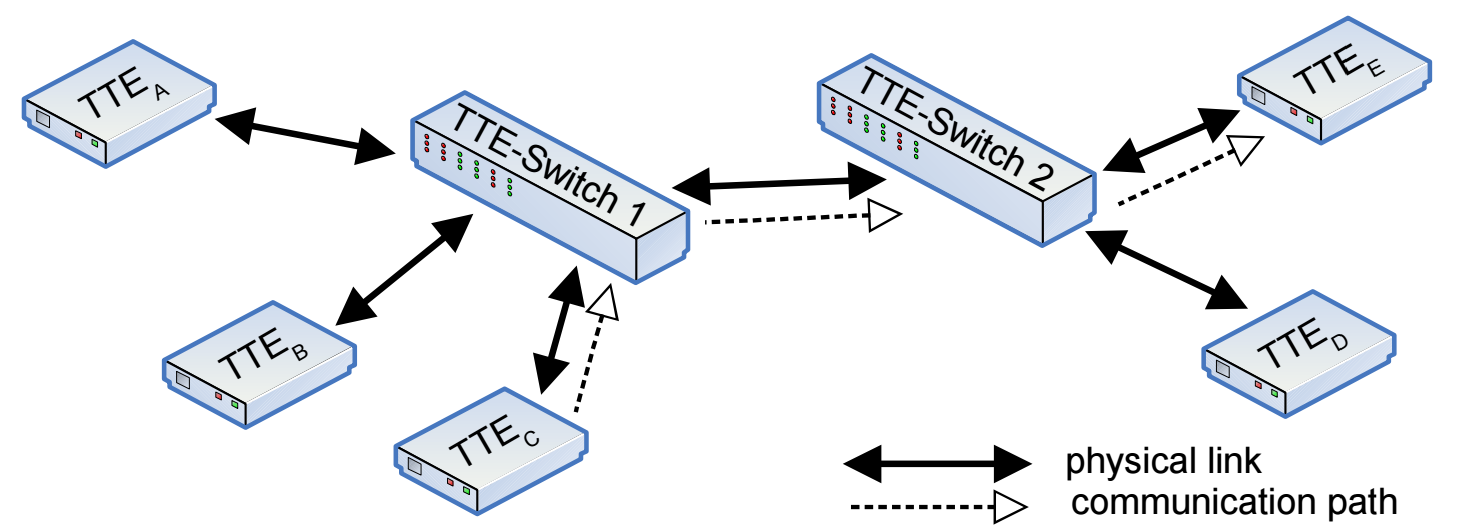
\includegraphics[width=12cm]{imgs/png/stateOfTheArt_2_TTEthernetNetwork.png}
    \caption{Example of TTEthernet network with 5 end-systems and 2 switches (extracted from~\cite{Craciunas2016}).}
    \label{fig_stateOfTheArt_2_TTEthernetNetwork}
\end{figure}
Although applied to macroscopic-sized networked systems such as the one depicted in Figure~\ref{fig_stateOfTheArt_2_TTEthernetNetwork}, the work of Craciunas \etal~\cite{Craciunas2016} shares many common aspects with our problem. They propose to compute simultaneously the schedules of tasks on end-systems and the schedules of communications over the virtual channels of a \emph{TTEthernet} network~\cite{ttethernet} using \emph{Satisfiability Modulo Theories} (or \emph{SMT}) and \emph{Mixed Integer Programming} (or \emph{MIP}) solvers. When focusing on many-core processors, the scheduling problem falls in a somewhat similar category where both tasks' and communications' schedule are inter-dependent. Unfortunately, the approach presented in~\cite{Craciunas2016} only partially solves our problem. The authors focus on a pure \emph{scheduling} issue to answer the question of \emph{when} tasks and communications are executed. The \emph{mapping} problem to decide \emph{where} should each task be assigned is not relevant in their context since the function of each end-system is assumed to be known a priori. In our case, no such pre-assignment of tasks to cores is comprised into the model. Therefore, a pre-mapping technique is required to apply the method. However, one may note that splitting the global problem into two sub-problems of mapping and scheduling solved sequentially does not allow to cover the whole solution space. 

\section{Summary}

In this chapter, we overviewed the various methods that where proposed to map and schedule dependent tasksets on distributed and many-core architectures. We identified in the DAG task model many similarities with our application model. Unfortunately, most of previous works regarding this model either focus on on-line scheduling techniques or are hardly directly applicable to a real-time context, to a many-core architecture or to an industrial context. We overviewed several other techniques focusing on hard-real time scheduling on many-core processors, including approaches targeting the \mppalong. While these approaches show promising results regarding the utilizability of many-core processors in real-time systems, none considers simultaneously an application model similar to ours together with the aerospace and industrial constraints we previously described in Chapter~\ref{chap_systemModel}. The second axis of contribution of this thesis is thus a novel mapping and scheduling technique solving both issues at once.

\clearpage
\subbiblio
\end{document}
